\section{等式QP的求解}
\label{sec:sqp-equality-qp}

式~\eqref{eq:sqp-qp}只含等式时，怎样求出它的解，这个解又在什么条件下才算数？这是SQP最基本的一步，下一节处理不等式时，每一轮要解的也是这种问题。为减少上标，本节在不引起混淆时省去$(t)$，并记$\bm{g}=\nabla f(\bm{x}^{(t)})$。

\paragraph{KKT线性系统}
只含等式时，条件~\eqref{eq:sqp-qp-kkt}的第一、二行就是全部要求。它们对$(\bm{d},\hat{\bm{\nu}})$是线性的，合起来写成块方程
\begin{equation}
 \underbrace{\begin{bmatrix}\bm{B}&\bm{A}^\top\\\bm{A}&\bm{0}\end{bmatrix}}_{\bm{K}}
 \begin{bmatrix}\bm{d}\\\hat{\bm{\nu}}\end{bmatrix}
 =-\begin{bmatrix}\bm{g}\\\bm{h}\end{bmatrix}.
 \label{eq:sqp-kkt-system}
\end{equation}
矩阵$\bm{K}\in\mathbb{R}^{(n+p)\times(n+p)}$称为\term{KKT矩阵}（KKT matrix）。它对称但不定，零对角块使它不可能正定，所以不能用Cholesky分解。

这个方程有解并不等于模型有最小点。要回答后一个问题，得看$\bm{B}$在允许的方向上是否向上弯。允许的方向是满足$\bm{A}\bm{v}=\bm{0}$的方向，它们构成$\bm{A}$的零空间。取矩阵$\bm{Z}\in\mathbb{R}^{n\times(n-p)}$，其各列构成这个零空间的一组基，就把问题缩到这$n-p$维上。矩阵$\bm{Z}^\top\bm{B}\bm{Z}$称为\term{约化Hessian}（reduced Hessian）。

\begin{theorem}[等式QP的可解性]
\label{thm:sqp-eqp}
设$\bm{A}\in\mathbb{R}^{p\times n}$行满秩，$\bm{Z}$的各列是其零空间的一组基，且$\bm{Z}^\top\bm{B}\bm{Z}\succ\bm{0}$。则$\bm{K}$可逆，方程~\eqref{eq:sqp-kkt-system}有唯一解$(\bm{d},\hat{\bm{\nu}})$，并且$\bm{d}$是等式QP唯一的全局最小点。
\end{theorem}

\begin{proof}
先证$\bm{K}$可逆。设$\bm{K}(\bm{u}^\top,\bm{w}^\top)^\top=\bm{0}$，即$\bm{B}\bm{u}+\bm{A}^\top\bm{w}=\bm{0}$且$\bm{A}\bm{u}=\bm{0}$。

用$\bm{u}^\top$左乘第一式，并用$\bm{A}\bm{u}=\bm{0}$消去含$\bm{w}$的项，得到
\[
 \bm{u}^\top\bm{B}\bm{u}=0.
\]

由$\bm{A}\bm{u}=\bm{0}$可写$\bm{u}=\bm{Z}\bm{z}$，代入上式得到
\[
 \bm{z}^\top\bm{Z}^\top\bm{B}\bm{Z}\bm{z}=0.
\]

约化Hessian正定，所以$\bm{z}$和$\bm{u}$都是零向量。第一式于是成为$\bm{A}^\top\bm{w}=\bm{0}$，$\bm{A}$行满秩给出$\bm{w}=\bm{0}$。

再证最小性。设$\bar{\bm{d}}$是任一可行步，令$\bm{v}=\bar{\bm{d}}-\bm{d}$，则$\bm{A}\bm{v}=\bm{0}$。记目标为$q$，展开得
\[
 q(\bar{\bm{d}})-q(\bm{d})=\langle\bm{g}+\bm{B}\bm{d},\bm{v}\rangle+\frac12\bm{v}^\top\bm{B}\bm{v}.
\]

由方程第一行，$\bm{g}+\bm{B}\bm{d}=-\bm{A}^\top\hat{\bm{\nu}}$，它与$\bm{v}$正交，第一项为零。所以
\[
 q(\bar{\bm{d}})-q(\bm{d})=\frac12\bm{v}^\top\bm{B}\bm{v}.
\]
$\bm{v}\neq\bm{0}$时$\bm{v}=\bm{Z}\bm{z}$且$\bm{z}\neq\bm{0}$，右端为正。
\end{proof}

两个条件各有分工。行满秩保证约束不互相矛盾、乘子唯一：若$\bm{A}$有一行是另一行的倍数而右端不相称，线性化约束根本无解，这种情形留到第~\ref{sec:sqp-restoration}节。约化Hessian正定保证驻点是最小点，它只要求$\bm{B}$在$n-p$个允许的方向上正定，不要求$\bm{B}$在全空间正定，第~\ref{sec:sqp-curvature}节会看到两者的差别。

\paragraph{直接解鞍点方程}
第一种做法是把$\bm{K}$当作一个$(n+p)$阶的对称不定矩阵，做带主元的$\bm{L}\bm{D}\bm{L}^\top$分解后回代。它一次同时给出$\bm{d}$和$\hat{\bm{\nu}}$，也能保持稀疏性，是大规模稀疏问题的常用选择。

小问题可以手算，办法是先消去$\bm{d}$。回到第一个模型，取$\bm{\nu}^{(0)}=1$，于是$\bm{B}=2\nu^{(0)}\bm{I}=2\bm{I}$，数据是
\[
 \bm{g}=(-1,-1)^\top,\qquad h=0.5,\qquad \bm{A}=(3,1).
\]

方程~\eqref{eq:sqp-kkt-system}的第一行给出$\bm{d}$关于$\hat\nu$的表达式：
\[
 \bm{d}=-\frac12\bigl(\bm{g}+\hat\nu\bm{A}^\top\bigr)=\frac12\begin{bmatrix}1-3\hat\nu\\1-\hat\nu\end{bmatrix}.
\]

代入第二行$\bm{A}\bm{d}=-h$，左端是$\frac12(3-9\hat\nu+1-\hat\nu)=2-5\hat\nu$，于是
\[
 2-5\hat\nu=-0.5,\qquad\text{即}\qquad\hat\nu=0.5.
\]

再代回$\bm{d}$的表达式，得到
\[
 \bm{d}=(-0.25,\ 0.25)^\top.
\]
这就是图~\ref{fig:sqp-circle-model}中的绿色箭头。

\paragraph{在零空间中求解}
第二种做法把步分成两段，分别完成两件事。第一段让线性化约束成立，第二段在不破坏它的前提下降低模型。取$\bm{Y}\in\mathbb{R}^{n\times p}$使$\bm{A}\bm{Y}$可逆，把步写成
\begin{equation}
 \bm{d}=\bm{Y}\bm{d}_Y+\bm{Z}\bm{d}_Z.
 \label{eq:sqp-range-null}
\end{equation}

因为$\bm{A}\bm{Z}=\bm{0}$，约束$\bm{A}\bm{d}=-\bm{h}$只约束$\bm{d}_Y$，得到$p$维的方程
\begin{equation}
 \bm{A}\bm{Y}\bm{d}_Y=-\bm{h}.
 \label{eq:sqp-normal-step}
\end{equation}

固定$\bm{d}_Y$，把式~\eqref{eq:sqp-range-null}代入目标，对$\bm{d}_Z$求最小，就是$n-p$维的无约束二次问题，其驻点方程为
\begin{equation}
 \bm{Z}^\top\bm{B}\bm{Z}\,\bm{d}_Z=-\bm{Z}^\top\bigl(\bm{g}+\bm{B}\bm{Y}\bm{d}_Y\bigr).
 \label{eq:sqp-reduced-step}
\end{equation}

最后，方程~\eqref{eq:sqp-kkt-system}的第一行左乘$\bm{Y}^\top$，就解出乘子：
\begin{equation}
 (\bm{A}\bm{Y})^\top\hat{\bm{\nu}}=-\bm{Y}^\top\bigl(\bm{g}+\bm{B}\bm{d}\bigr).
 \label{eq:sqp-null-multiplier}
\end{equation}

继续用同一组数据。取$\bm{Y}=\bm{A}^\top=(3,1)^\top$，此时$\bm{A}\bm{Y}=10$，再取$\bm{Z}=(1,-3)^\top$，可以核对$\bm{A}\bm{Z}=0$。由式~\eqref{eq:sqp-normal-step}，
\[
 d_Y=-\frac{0.5}{10}=-0.05,\qquad \bm{Y}d_Y=(-0.15,\ -0.05)^\top.
\]

计算式~\eqref{eq:sqp-reduced-step}的两边。约化Hessian是$\bm{Z}^\top\bm{B}\bm{Z}=2\times10=20$，右端需要的向量和内积是
\[
 \bm{g}+\bm{B}\bm{Y}d_Y=(-1.3,\ -1.1)^\top,\qquad
 \bm{Z}^\top(\bm{g}+\bm{B}\bm{Y}d_Y)=-1.3+3.3=2.
\]

于是
\[
 d_Z=-\frac{2}{20}=-0.1,\qquad \bm{Z}d_Z=(-0.1,\ 0.3)^\top.
\]

两段相加，得到$\bm{d}=(-0.25,0.25)^\top$，和直接解法一致。用式~\eqref{eq:sqp-null-multiplier}求乘子，先算$\bm{g}+\bm{B}\bm{d}=(-1.5,-0.5)^\top$，于是
\[
 10\,\hat\nu=-(3,1)\begin{bmatrix}-1.5\\-0.5\end{bmatrix}=5,\qquad\hat\nu=0.5.
\]

图~\ref{fig:sqp-range-null}是这两段的几何。紫色的一段垂直于虚线，它只管把点送到线性化约束上；黄色的一段沿虚线走，它只管沿允许的方向降低模型，这里的$\bm{Z}$就是把“沿虚线走多少”变成$\mathbb{R}^2$中位移的那个矩阵。

\begin{BookInlineFigure}
 \centering
 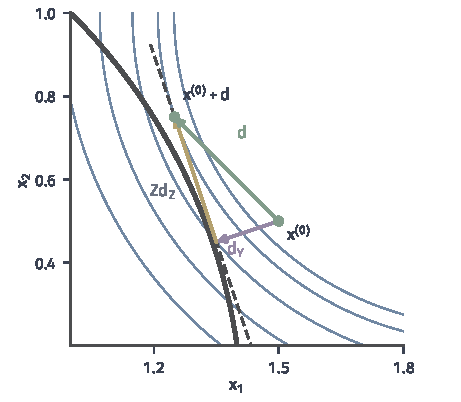
\includegraphics[width=78mm]{figures/05-optimization/06-constrained-optimization/matplotlib/sqp-range-null/figure.pdf}
 \caption{第一个局部模型的两段分解。深灰粗线是圆，虚线是线性化约束，蓝线是模型的等值线。紫色$\bm{Y}d_Y$从$\bm{x}^{(0)}$走到虚线，黄色$\bm{Z}d_Z$沿虚线走到模型的条件最小点，两段之和是绿色的$\bm{d}$。}
 \label{fig:sqp-range-null}
\end{BookInlineFigure}

\begin{BookInlineTable}
 \centering
 \begin{tabular}{lll}
  \toprule
  比较项 & 解KKT系统 & 零空间方法\\
  \midrule
  分解对象 & $(n+p)$阶对称不定 & $\bm{A}$的分解与$n-p$阶约化矩阵\\
  $n-p$很小时 & 仍解$n+p$阶 & 约化矩阵很小，便宜\\
  稀疏性 & 容易保持 & $\bm{Z}$可能变稠密\\
  检查曲率 & 需看分解的惯性 & 直接检查约化矩阵\\
  \bottomrule
 \end{tabular}
 \caption{等式QP两种解法的比较。}
 \label{tab:sqp-eqp-methods}
\end{BookInlineTable}

\paragraph{与原问题Newton步的关系}
到这里，KKT系统还只是模型的条件。现在换一个角度，从原问题出发。只含等式时，原问题的KKT条件是非线性方程组
\begin{equation}
 \bm{F}(\bm{x},\bm{\nu})=\begin{bmatrix}\nabla f(\bm{x})+\bm{A}(\bm{x})^\top\bm{\nu}\\\bm{h}(\bm{x})\end{bmatrix}=\bm{0}.
 \label{eq:sqp-kkt-map}
\end{equation}
自然的想法是对这个方程组直接用Newton法。下面的定理说，这和解局部QP是同一件事。

\begin{theorem}[SQP与KKT方程的Newton法]
\label{thm:sqp-newton}
设$\bm{B}$取Lagrange函数在$(\bm{x},\bm{\nu})$处对$\bm{x}$的Hessian。则$(\bm{\delta}_x,\bm{\delta}_\nu)$是$\bm{F}$在$(\bm{x},\bm{\nu})$处的Newton步，当且仅当$\bm{d}=\bm{\delta}_x$，$\hat{\bm{\nu}}=\bm{\nu}+\bm{\delta}_\nu$满足方程~\eqref{eq:sqp-kkt-system}。
\end{theorem}

\begin{proof}
$\bm{F}$的第一块对$\bm{x}$的导数是$\nabla^2_{\bm{x}\bm{x}}\mathcal{L}=\bm{B}$，对$\bm{\nu}$的导数是$\bm{A}^\top$；第二块对$\bm{x}$的导数是$\bm{A}$，对$\bm{\nu}$的导数为零。所以Newton方程是
\[
 \begin{bmatrix}\bm{B}&\bm{A}^\top\\\bm{A}&\bm{0}\end{bmatrix}
 \begin{bmatrix}\bm{\delta}_x\\\bm{\delta}_\nu\end{bmatrix}
 =-\begin{bmatrix}\bm{g}+\bm{A}^\top\bm{\nu}\\\bm{h}\end{bmatrix}.
\]

第一行把右端的$-\bm{A}^\top\bm{\nu}$移到左边，与$\bm{A}^\top\bm{\delta}_\nu$合并成$\bm{A}^\top(\bm{\nu}+\bm{\delta}_\nu)$，就得到方程~\eqref{eq:sqp-kkt-system}。每一步都可逆，反过来也成立。
\end{proof}

定理给出了两种读法。模型的读法是“在切平面上最小化一个二次函数”，Newton的读法是“解KKT这组方程”。前者告诉我们什么时候解是最小点，后者告诉我们为什么收敛快。两种读法也有差别：Newton法只求方程的根，不区分极小点和极大点；模型的读法多出了约化曲率这一判据。

\paragraph{计算过程}
下面把等式约束的SQP用问题~\eqref{eq:sqp-circle}完整走几轮。这里用精确的Lagrange Hessian和全步长，$\alpha^{(t)}=1$，步的接受规则留到第~\ref{sec:sqp-acceptance}节。

\needspace{6\baselineskip}
\paragraph{变量}
\begin{itemize}
 \item $\bm{x}^{(t)}\in\mathbb{R}^n$：当前点，例中$n=2$。
 \item $\bm{\nu}^{(t)}\in\mathbb{R}^p$：当前乘子估计，例中$p=1$。
 \item $\bm{g}^{(t)}\in\mathbb{R}^n$、$\bm{h}^{(t)}\in\mathbb{R}^p$：目标梯度与约束值。
 \item $\bm{A}^{(t)}\in\mathbb{R}^{p\times n}$：约束Jacobian，例中是$1\times2$的行向量。
 \item $\bm{B}^{(t)}\in\mathbb{R}^{n\times n}$：Lagrange Hessian，例中为$2\nu^{(t)}\bm{I}$。
 \item $\bm{d}^{(t)}\in\mathbb{R}^n$、$\hat{\bm{\nu}}\in\mathbb{R}^p$：子问题的解与乘子。
\end{itemize}

\paragraph{初始化}
给定$\bm{x}^{(0)}$和$\bm{\nu}^{(0)}$，以及精度$\varepsilon>0$。例中
\[
 \bm{x}^{(0)}=(1.5,\ 0.5)^\top,\qquad \nu^{(0)}=1,\qquad\varepsilon=10^{-10}.
\]

\needspace{6\baselineskip}
\paragraph{每轮更新}
\begin{enumerate}
 \item 在$\bm{x}^{(t)}$处计算$\bm{g}^{(t)},\bm{h}^{(t)},\bm{A}^{(t)}$，并由式~\eqref{eq:sqp-lagrangian-hessian}计算$\bm{B}^{(t)}$。

 例中第一轮的数值已算过。第二轮$\bm{x}^{(1)}=(1.25,0.75)^\top$，$\nu^{(1)}=0.5$，数据是
 \[
  \bm{g}^{(1)}=(-1,-1)^\top,\quad h^{(1)}=0.125,\quad\bm{A}^{(1)}=(2.5,1.5),\quad\bm{B}^{(1)}=\bm{I}.
 \]

 \item 解方程~\eqref{eq:sqp-kkt-system}得$\bm{d}^{(t)}$和$\hat{\bm{\nu}}$。$\bm{K}$可逆时，它们的显式形式是
 \begin{equation}
  \begin{bmatrix}\bm{d}^{(t)}\\\hat{\bm{\nu}}\end{bmatrix}
  =-\bigl(\bm{K}^{(t)}\bigr)^{-1}\begin{bmatrix}\bm{g}^{(t)}\\\bm{h}^{(t)}\end{bmatrix}.
  \label{eq:sqp-full-step}
 \end{equation}

 例中第一轮得$\bm{d}^{(0)}=(-0.25,0.25)^\top$，$\hat\nu=0.5$。第二轮由第一行$\bm{d}=\bm{e}-\hat\nu\bm{A}^\top$，其中$\bm{e}=(1,1)^\top$，代入第二行得
 \[
  4-8.5\,\hat\nu=-0.125,\qquad\hat\nu=\frac{33}{68}\approx0.48529.
 \]

 代回第一行，得到
 \[
  \bm{d}^{(1)}\approx(-0.21324,\ 0.27206)^\top.
 \]

 \item 更新迭代点和乘子：
 \begin{equation}
  \bm{x}^{(t+1)}=\bm{x}^{(t)}+\bm{d}^{(t)},\qquad\bm{\nu}^{(t+1)}=\hat{\bm{\nu}}.
  \label{eq:sqp-full-update}
 \end{equation}

 例中前两轮得到
 \[
  \bm{x}^{(1)}=(1.25,\ 0.75)^\top,\qquad\bm{x}^{(2)}\approx(1.03676,\ 1.02206)^\top.
 \]

 第三轮的数据是$h^{(2)}\approx0.11949$，$\bm{A}^{(2)}\approx(2.07353,2.04412)$，$\bm{B}^{(2)}\approx0.97059\,\bm{I}$，同样解方程得
 \[
  \hat\nu\approx0.49937,\qquad\bm{d}^{(2)}\approx(-0.03653,\ -0.02140)^\top.
 \]

 \item 若下面两个残差都不超过$\varepsilon$，就停止，否则回到第1步：
 \[
  \lVert\bm{g}^{(t)}+(\bm{A}^{(t)})^\top\bm{\nu}^{(t)}\rVert_2,\qquad\lVert\bm{h}^{(t)}\rVert_2.
 \]
 例中在$t=5$时停止。
\end{enumerate}

最终得到$\bm{x}^{(5)}\approx(1,1)^\top$，$\nu^{(5)}\approx0.5$。表~\ref{tab:sqp-newton-run}列出各轮结果，图~\ref{fig:sqp-newton-path}画出路径与残差。

\begin{BookInlineTable}
 \centering
 \begin{tabular}{rlllll}
  \toprule
  $t$ & $x_1^{(t)}$ & $x_2^{(t)}$ & $\nu^{(t)}$ & $\lvert h^{(t)}\rvert$ & $\lVert\bm{x}^{(t)}-\bm{x}^\star\rVert_2$\\
  \midrule
  0 & 1.5 & 0.5 & 1 & 0.5 & $7.07\times10^{-1}$\\
  1 & 1.25 & 0.75 & 0.5 & 0.125 & $3.54\times10^{-1}$\\
  2 & 1.03676 & 1.02206 & 0.48529 & 0.11949 & $4.29\times10^{-2}$\\
  3 & 1.00024 & 1.00066 & 0.49937 & $1.79\times10^{-3}$ & $7.02\times10^{-4}$\\
  4 & 1.00000 & 1.00000 & 0.50000 & $4.9\times10^{-7}$ & $4.19\times10^{-7}$\\
  5 & 1.00000 & 1.00000 & 0.50000 & $<10^{-12}$ & $2.69\times10^{-13}$\\
  \bottomrule
 \end{tabular}
 \caption{问题~\eqref{eq:sqp-circle}上全步长SQP的各轮结果。}
 \label{tab:sqp-newton-run}
\end{BookInlineTable}

\begin{BookInlineFigure}
 \centering
 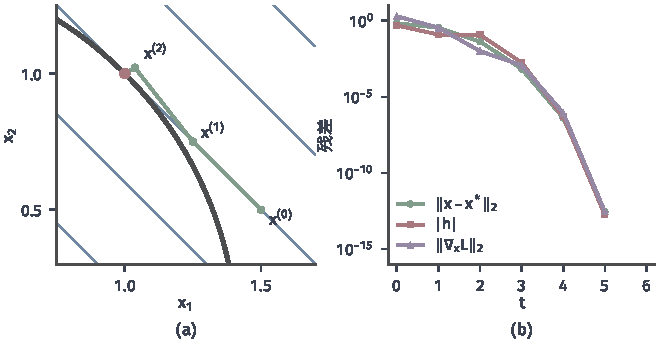
\includegraphics[width=112mm]{figures/05-optimization/06-constrained-optimization/matplotlib/sqp-newton-path/figure.pdf}
 \caption{问题~\eqref{eq:sqp-circle}上全步长SQP的运行结果。(a)~路径（绿），中间各点都不在圆上。(b)~到解的距离、约束残差和Lagrange梯度随迭代的变化，纵轴为对数，后几轮每步的有效数字大致翻倍。}
 \label{fig:sqp-newton-path}
\end{BookInlineFigure}

表中有两点值得注意。第一，约束残差的下降并不均匀，$t=1$到$t=2$几乎没有变化，因为这一步走得长，二阶误差$\lVert\bm{d}\rVert_2^2$把线性化的好处抵消了。第二，从$t=2$起误差大致平方下降，这是Newton型方法的标志，第~\ref{sec:sqp-convergence}节给出证明。
